\documentclass[11pt,a4paper]{article}
\usepackage{graphicx}
\usepackage{amssymb, amsmath}
\usepackage{url}
\usepackage{polski}
\usepackage{subfigure}
\usepackage[utf8]{inputenc} 

\title{Współczesne techniki heurystyczne\\ Sprawozdanie nr 2.\\ \large Zastosowanie algorytmu rozmytego do sterowania prędkością samochodu}
\author{Piotr Jastrzębski\\ Marcin Nazimek}
\date{}
\begin{document}
\maketitle

\section{Szczegółowy opis zadania}\label{opis}
Rozważmy poruszający się samochód. W celu stworzenia modelu ruchu bierzemy pod uwagę dwie zmienne wejściowe: PRĘDKOŚĆ i ODLEGŁOŚĆ od jadącego z przodu samochodu oraz jedna zmienna określająca zmianę tego ruchu PRZYSPIESZENIE. Sterowanie odbywać będzie się poprzez zmianę prędkości. Przykładowe możliwe stany to: przyspieszenie, utrzymanie prędkości i hamowanie (ale można przyjąć więcej stanów, np. odległość jest bardzo mała, itp.).

Dla rozpatrywanego przypadku, baza reguł ma postać:
\begin{itemize}
\item IF odległość jest mała AND prędkość jest mała THEN utrzymaj prędkość.
\item IF odległość jest mała AND prędkość jest duża THEN zredukuj prędkość.
\item IF odległość jest duża AND prędkość jest mała THEN zwiększaj prędkość.
\item IF odległość jest duża AND prędkość jest duża THEN utrzymaj prędkość.
\end{itemize}
Zmienne ODLEGŁOŚĆ, PRĘDKOŚĆ i PRZYSPIESZENIE to zmienne lingwistyczne, które mogą przyjmować rozmyte wartości: krótki, długi, mała, duża, utrzymaj, zredukuj i zwiększaj. Projektant ma teraz za zadanie dobrać tak parametry zbiorów rozmytych i obszarów rozważań by odpowiadały one rzeczywistości w jak najlepszym stopniu.

\section{Założenia projektu}\label{zalozenia}
Projekt ma symulować i prezentować wykorzystanie algorytmu logiki rozmytej do sterowania prędkością samochodu w~możliwie największym stopniu odwzorowując rzeczywistość.

W przygotowanym środowisku na potrzeby prezentacji wykorzystane są dwa uproszczone modele reprezentujące samochody -- pierwszy, dalej oznaczany jako $A$, będący samochodem, dla którego przygotowane zostanie sterowanie, oraz samochód $B$, który w sposób niedeterministyczny, ale zgodny z przepisami i realnymi wartościami przyspieszeń, będzie poruszał się przed $A$. Każdy z nich w~danej chwili czasu opisany będzie prędkością bezwzględną. 

Odległość między samochodami wynika wprost z różnic prędkości, a prędkość auta $A$ modyfikowana jest przez wartość wyjścia modułu logiki rozmytej -- przyspieszeniem.

\subsection{Ograniczenia}
Na potrzeby projektu przyjęto następujące ograniczenia:
\begin{itemize}
\item \textbf{Prędkość} - przyjmuje wartości z zakresu $0\div140km/h$ \footnote{Założono, że ruch odbywa się na autostradzie w Polsce.}.
\item \textbf{Przyspieszenie} - jest zmienne w czasie. Kwestią do rozstrzygnięcia pozostaje, czy będzie ono takie samo czy przyjmie różne wartości dla opóźnienia i przyspieszenia. Na bazie zgromadzonych informacji odpowiednie wydaje się przyjęcie wartości przyspieszenia z zakresu $\langle-9\frac{m}{s^2};4\frac{m}{s^2}\rangle$\footnote{Wartości prawdziwe dla suchej nawierzchni.} i~dla aktualnego stanu zaawansowania projektu takie jest wykorzystywane.
\item \textbf{Odległość} - wyrażona w kilometrach dowolną nieujemną liczbą dziesiętną. Testowane jest rozwiązanie, które rozważa niejako dwa stany:
	\begin{itemize}
		\item stan bliski -- do odległości $1 km$, gdzie aktywny jest moduł logiki rozmytej
		\item stan daleki -- powyżej $1km$, gdzie samochód porusza się prędkością autostradową, tak długo, aż nie na trafi w odległości $1 km$ ma poprzedzające auto. Tym samym wartość $1 km$ jest wartością rozgraniczającą niejako nieskończoność od skutecznej odległości działania modułu dystansującego.
	\end{itemize}
\end{itemize}
Każde przekroczenie wartości $0$ świadczy o najechaniu na samochód poprzedzający i~w~końcowej wersji projektu nie ma prawa wystąpić.

\subsection{Stan początkowy}
Przed rozpoczęciem symulacji stan układu (wartości poszczególnych parametrów) mogą być modyfikowane. Ustalane mogą być zarówno prędkość początkowa samochodu $A$ oraz $B$ jak i odległość między nimi. Celem symulacji jest tak sterować parametrami samochodu $A$, aby zachowywał on stałą odległość od poprzedzającego go samochodu nie powodując kolizji (najechania). Aktualnie zaimplementowana funkcjonalność pozwala na dowolne sterowanie prędkością samochodu poprzedzającego.

\subsection{Implementacja}
W celu prezentacji działania algorytmu wykorzystywane są funkcjonalności zawarte w programie \emph{Matlab R2011a} wraz z rozszerzeniem \emph{Fuzzy Logic Toolbox}. Moduł ten zapewnia funkcje, narzędzia graficzne i elementy \emph{Simulink} dla systemów bazujących na logice rozmytej. W aktualnie zaproponowanym rozwiązaniu bezwzględne prędkości aut prezentowane są na tym samym wykresie pozwalając obserwować proces reakcji samochodu sterowanego modułem logiki rozmytej.

\subsection{Aktualny postęp prac}
Jako początkowe założenie przyjęliśmy, że dwa stany odległości oraz prędkości oraz wynikające wprost z~nich cztery reguły decyzyjne wystarczą do wiernego symulowania procesu. Wydaje się jednak właściwe zwiększenie ich liczby i~np. odpowiedniejsze reagowanie na nagłe zatrzymanie (hamowanie awaryjne) samochodu poprzedzającego. W~toku dalszej pracy nad projektem takie przypadki zostaną sprawdzone.

W~międzyczasie wyklarowała się koncepcja prezentacji wyników symulacji. Wykorzystany został moduł \emph{Simulink}, który za pomocą kontrolera \emph{Fuzzy Logic Controller} oraz połączeń i sprzężeń zwrotnych realizuje zależności zmiennych między $A$ oraz $B$. Okazało się, że ze względu na specyfikę \emph{Matlaba}, konieczne jest wykorzystanie elementów opóźniających np. o~jeden takt w~celu eliminacji tzw.~\emph{Algebraic Loops}, co dobrze zostało wytłumaczone w \cite{simulink}. Nie wpływa to jednak na działanie programu. Do wyświetlania danych, m.in. wartości prędkości obu aut, odległości i przyspieszenia wykorzystane są elementy typu \emph{Display} oraz {Scope}. Pierwsze próby, przedstawione na rysunku \ref{img:simulink1}, sprawiły jednak spore problemy ze względu na brak możliwości wymuszenia taktu symulacji na predefiniowaną wartość np. jedną sekundę.

\subsection{Napotkane problemy}
Oprócz niemożności wymuszenia sekundowego taktowania, dość problematyczne wydaje się zachowanie modułu logiki rozmytej w~zależności od częstotliwości odświeżania stanu. Jak widać na rysunku \ref{img:tenToTwo} oraz \ref{img:tenToSix} jego zmiana silnie wpływa na oscylacje i~wygaszanie prędkości samochodu. Należy ten parametr dobierać rozważnie.

\begin{figure}
\centering
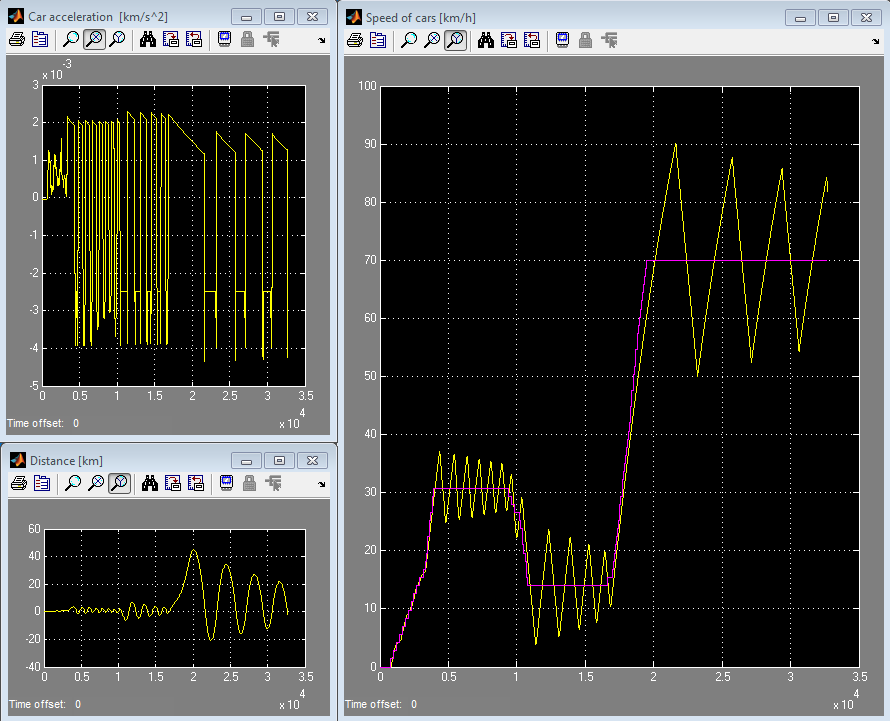
\includegraphics[width=0.8\textwidth]{10to2.png}
\caption{Wykresy parametrów samochodów przy 100 odświeżeń na sekundę stanu modułu Fuzzy Logic. (kolor żółty - samochód A, fioletowy - samochód B)} 
\label{img:tenToTwo}
\end{figure}

\begin{figure}
\centering
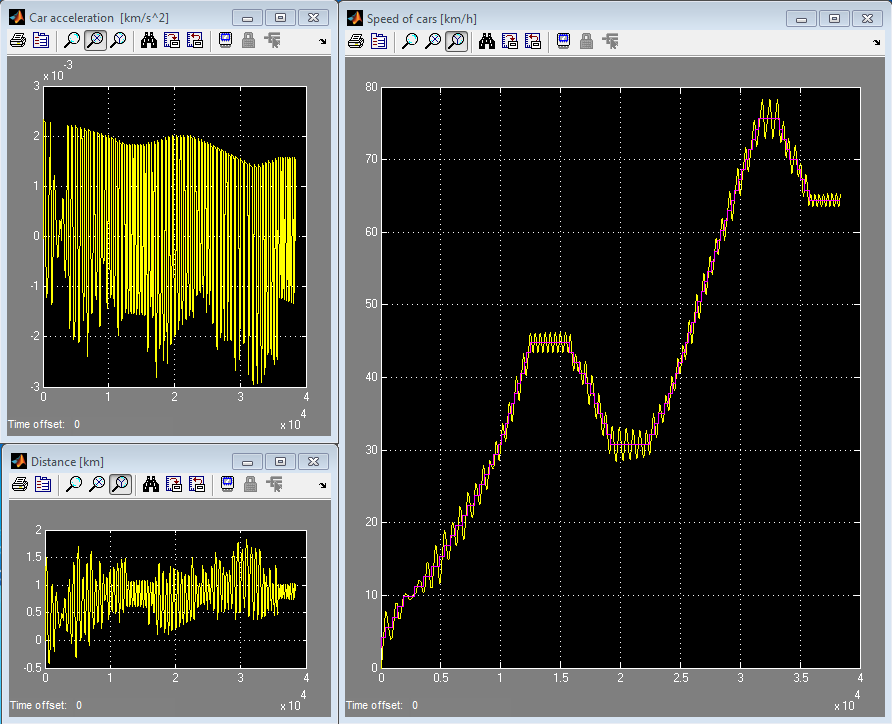
\includegraphics[width=0.8\textwidth]{10to6.png}
\caption{Wykresy parametrów samochodów przy 1000000 odświeżeń na sekundę stanu modułu Fuzzy Logic. (kolor żółty - samochód A, fioletowy - samochód B)} 
\label{img:tenToSix}
\end{figure}

\subsection{Aktualne wyniki}
\begin{figure}
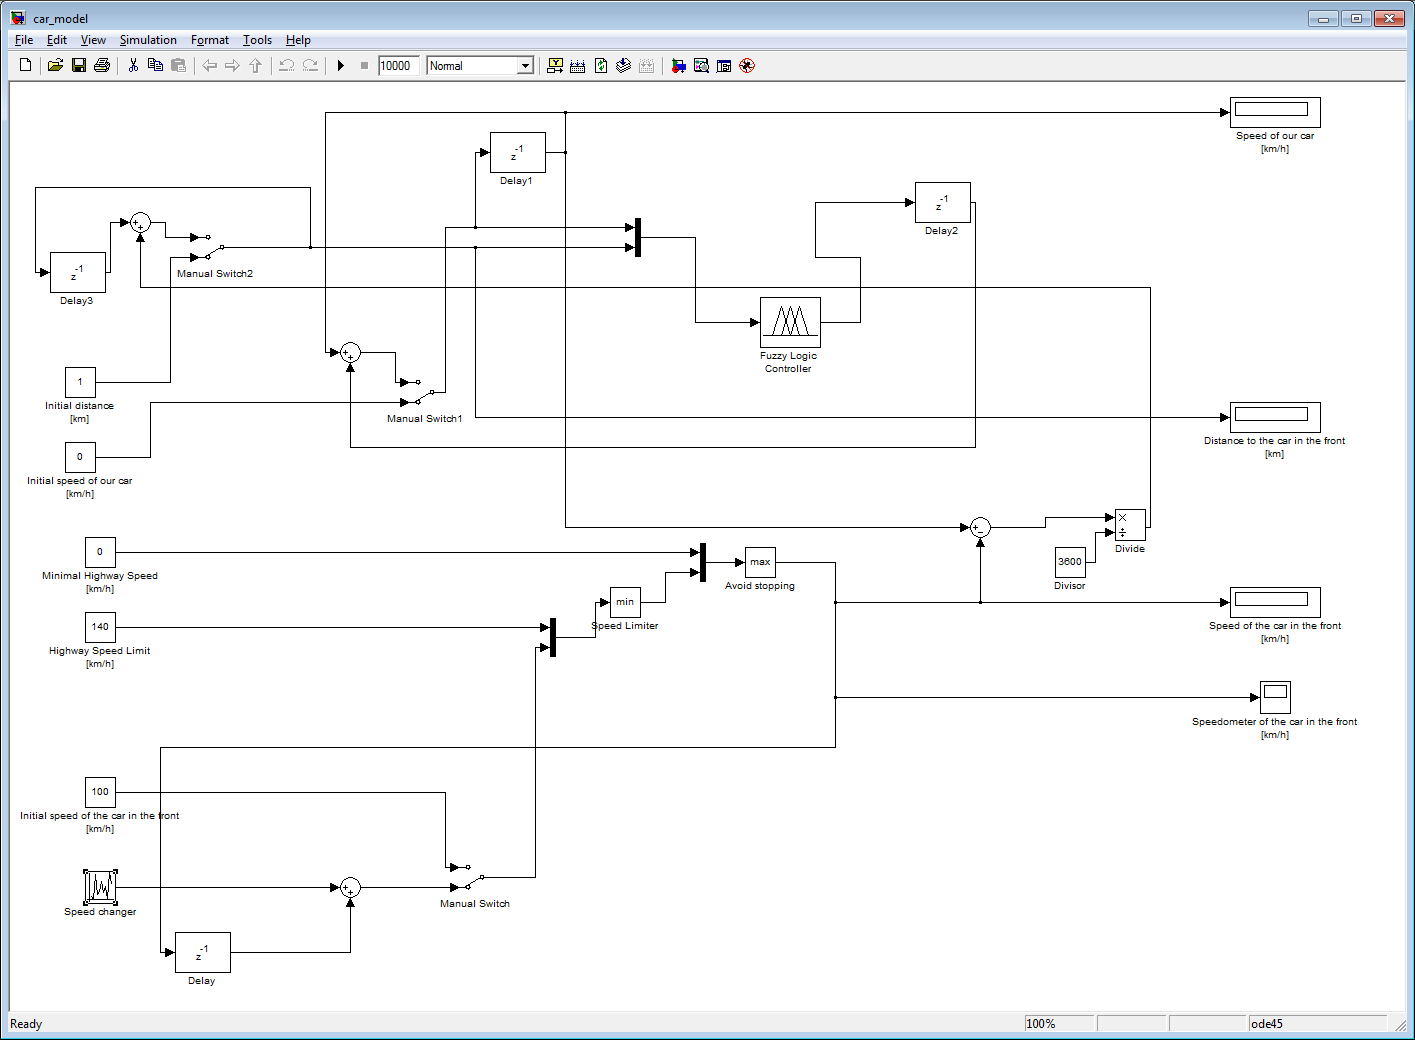
\includegraphics[width=\textwidth]{simulink1.png}
\caption{Wstępne, zarzucone już rozwiązanie w programie Simulink.} 
\label{img:simulink1}
\end{figure}

Aktualny stan zaawansowania pracy widoczny jest na rysunku \ref{img:simulink2} i~jest względem poprzedniej, całkowicie przeprojektowaną symulacją. Wyniki przeprowadzonych symulacji pokazują, że rozwiązanie zmierza w~dobrym kierunku. Dobierając parametry odświeżania modułu logiki rozmytej oraz modyfikując sam kontroler bez większego problemu do czasu finalnej wersji można uzyskać w~całości odpowiednio działający moduł sterowania samochodem. Przy aktualnej implementacji w~szczególnych warunkach zdarza się, że odległość między samochodami przyjmuje podczas oscylacji wartości ujemne, co w rzeczywistości skutkowałoby kolizją. Taka sytuacja nie może mieć miejsca. Moduł reaguje jednak poprawnie, steruje przewidywanie parametrami samochodu.

\begin{figure}
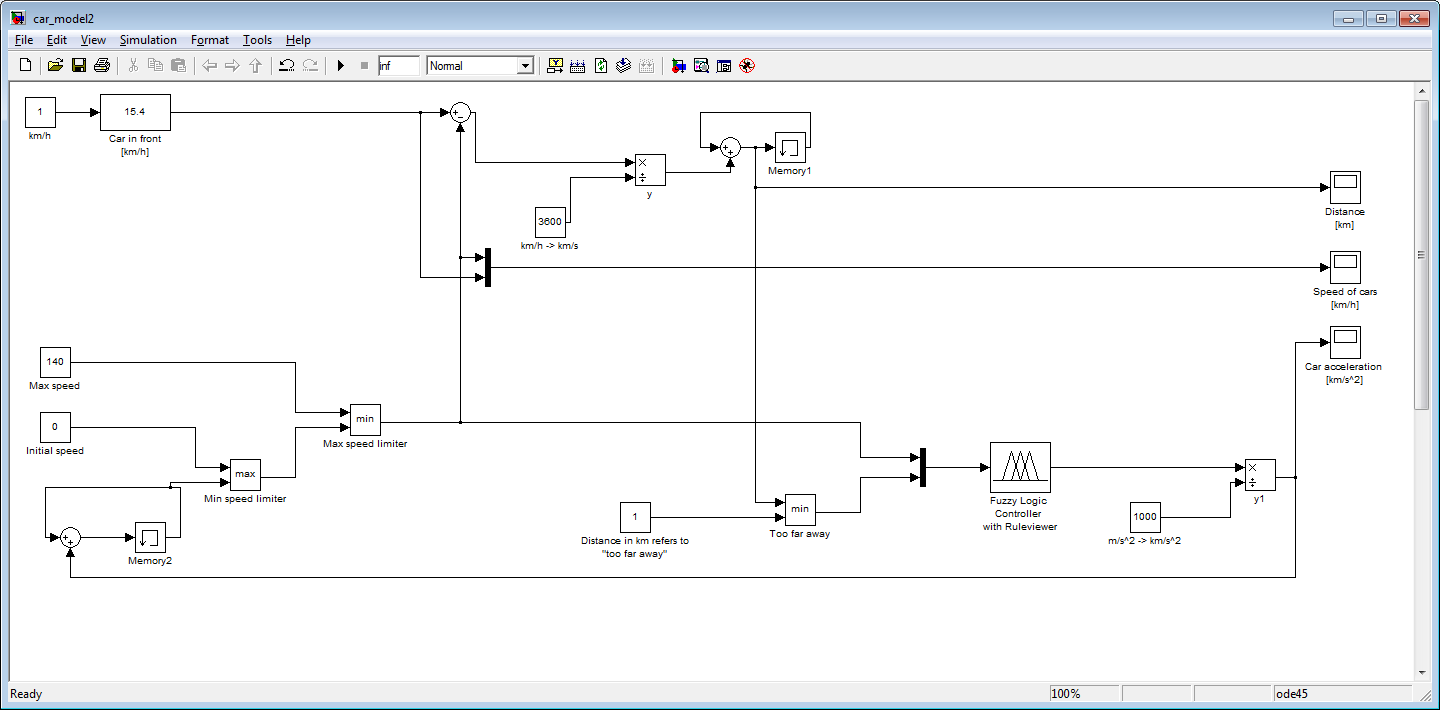
\includegraphics[width=\textwidth]{simulink2.png}
\caption{Rozwijane rozwiązanie w programie Simulink.} 
\label{img:simulink2}
\end{figure}

\subsection{Testowanie}
W przygotowanej wersji testowej samochód $B$ sterowany jest ręcznie, przez zmianę jego prędkości suwakiem, co znacznie ułatwia proces sprawdzania działania symulacji. W wersji końcowej kolizja będzie wykrywana, a~prędkość samochodu ,,uciekającego'' będzie automatycznie i~niedeterministycznie zmieniała się w czasie zachowując przyjęte wcześniej wartości przyspieszeń.

Dodatkowo, jak wspomniano wcześniej, sprawdzone zostaną różne kształty funkcji, jak na rysunku \ref{img:fuzzy} oraz przetestowane zostanie wykorzystanie większej liczby przedziałów odległości i~prędkości. Wyniki testów, po ich zakończeniu można obserwować na wykresach.

\begin{figure}
\label{img:fuzzy}
\centering
\mbox{
\subfigure[Funkcje trójkątne]{\label{img:x1}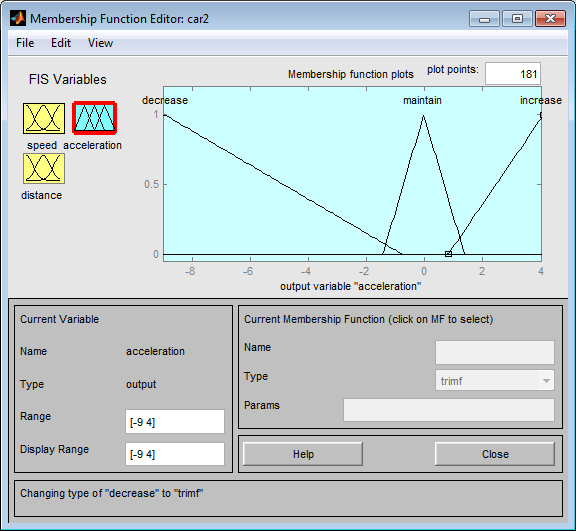
\includegraphics[width=0.40\textwidth]{fuzzy2.png}} \quad
\subfigure[Funkcje krzywych różnego stopnia]{\label{img:x2}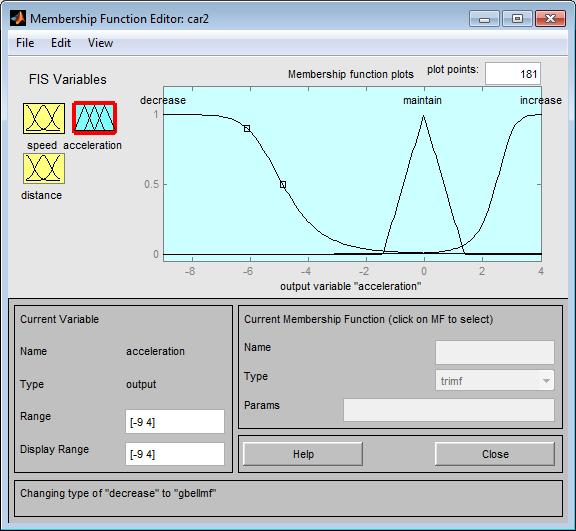
\includegraphics[width=0.40\textwidth]{fuzzy3.png}}
}
\mbox{
\subfigure[Funkcja trapezoidalne]{\label{img:x3}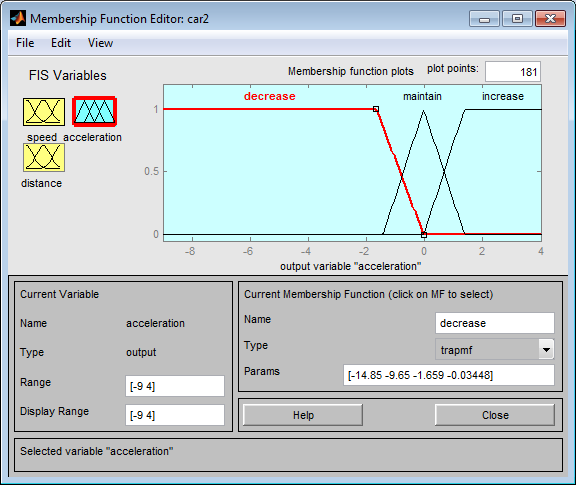
\includegraphics[width=0.40\textwidth]{fuzzy1.png}}\quad
\subfigure[Płaszczyzna przyspieszenia]{\label{img:x4}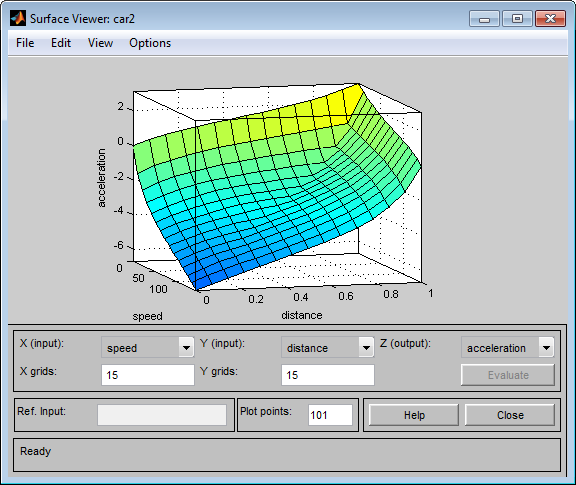
\includegraphics[width=0.40\textwidth]{fuzzy3d.png}} 
}
\caption{Porównanie przykładowych kształtów funkcji oraz płaszczyzny wartości przyspieszenia w zależności od prędkości i~odległości.}
\end{figure}

\begin{thebibliography}{9}
	\bibitem{manual}
	\emph{Fuzzy Logic Toolbox User’s Guide}\\
	\url{http://www.mathworks.com/help/pdf_doc/fuzzy/fuzzy.pdf}

	\bibitem{engApp}
	Ross T., \emph{Fuzzy Logic with Engineering Applications}

	\bibitem{opis}
	Rykaczewski K., \emph{Systemy rozmyte i ich zastosowania}\\
	\url{http://math.uni.lodz.pl/~fulmanp/zajecia/ssn/materialy/duszek.pdf}

	\bibitem{ieee1}
	Mamat M., Ghani N. M.,\emph{Fuzzy Logic Controller on Automated Car Braking System}, IEEE International Conference on Control and Automation, 2009. ICCA 2009. 

	\bibitem{ieee2}
	Khodayari, A., Kazemi, R., Ghaffari, A., Braunstingl, R., \emph{Design of an improved fuzzy logic based model for prediction of car following behavior}, IEEE International Conference on Mechatronics (ICM), 2011 

	\bibitem{ieee3}
	Sato, T., Akamatsu, M., Pengjun Zheng, McDonald, M., \emph{Comparison of car following behavior between UK and Japan}, ICCAS-SICE, 2009
	
	\bibitem{simulink}
	\emph{Simulating Dynamic Systems}\\
	\url{http://www.mathworks.com/help/simulink/ug/simulating-dynamic-systems.html}
\end{thebibliography}
\end{document}
